\documentclass[11pt]{article}
\usepackage[margin=1in]{geometry}
\usepackage{mathptmx}
\usepackage[T1]{fontenc}
\usepackage{booktabs,threeparttable,graphicx,placeins}
\usepackage[font=normalsize,labelfont=bf,skip=6pt]{caption}
\setlength{\parindent}{0pt}
\setlength{\textfloatsep}{14pt plus 2pt minus 2pt}
\setlength{\floatsep}{16pt plus 2pt minus 2pt}
\renewcommand{\topfraction}{0.95}
\renewcommand{\bottomfraction}{0.9}
\renewcommand{\textfraction}{0.05}
\renewcommand{\floatpagefraction}{0.8}
\title{Does RTI work? First-cut tables and figures}
\author{Amar and Sood}
\date{Data as of 29 October 2026}
\pdftrailerid{}
\begin{document}
\maketitle
\begin{table}[!htbp]
\centering
\caption{Sample and filing by state}
\label{tab:tab_sample}
\small
\begin{threeparttable}
\begin{tabular}{lrrrrrrl}
\toprule
State & Frame & Drawn & Plain / legal & Filed & Filed (\%) & Past day 30 & Filing window \\
\midrule
Tamil Nadu & 17,417 & 1,000 & 700 / 300 & 528 & 52.8 & 140 & 26 Aug to 28 Oct \\
Telangana & 3,401 & 375 & 262 / 113 & 218 & 58.1 & 187 & 04 Sep to 24 Oct \\
Karnataka & 1,800 & 180 & 126 / 54 & 149 & 82.8 & 78 & 11 Sep to 28 Oct \\
Delhi & 223 & 44 & 30 / 14 & 44 & 100.0 & 22 & 19 Sep to 26 Oct \\
Maharashtra & 328 & 66 & 46 / 20 & 61 & 92.4 & 28 & 15 Sep to 27 Oct \\
\midrule
All & 23,169 & 1,665 & 1,164 / 501 & 1,000 & 60.1 & 455 & 26 Aug to 28 Oct \\
\bottomrule
\end{tabular}
\begin{tablenotes}[flushleft]\footnotesize
\item \textit{Notes:} Data as of 29 October 2026. Past day 30: filed by 29 September, so the 30-day limit in s.7(1) has passed. Tamil Nadu is drawn by department $\times$ tier quotas, other states proportionally to department group with a cap.
\end{tablenotes}
\end{threeparttable}
\end{table}

\FloatBarrier
\begin{figure}[!htbp]
\centering
\caption{Cumulative filings by state}
\label{fig:fig_filings}
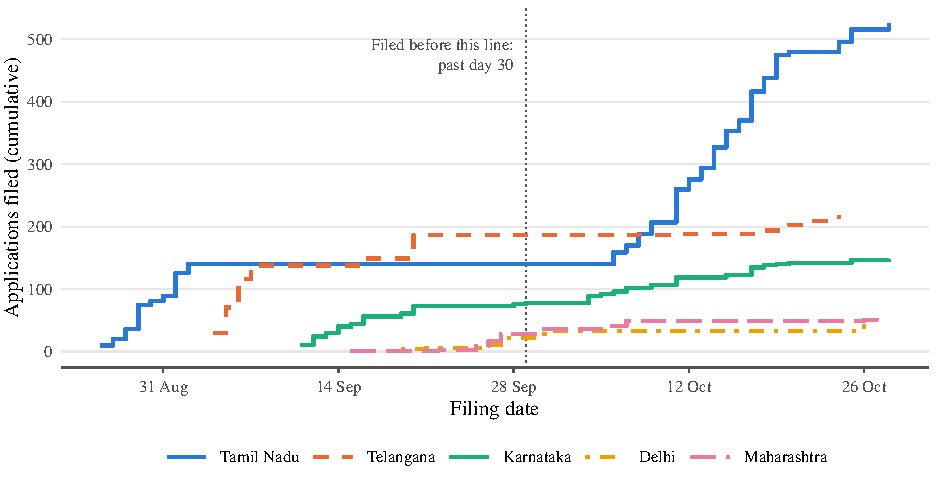
\includegraphics[width=\textwidth]{figures/fig_filings.pdf}
\begin{minipage}{\textwidth}\footnotesize
\textit{Notes:} One line per state; 999 applications have a filing date, from the portal acknowledgment where one exists, otherwise the RA sheet. Applications filed before the dotted line have passed the 30-day limit in s.7(1).
\end{minipage}
\end{figure}

\FloatBarrier
\begin{table}[!htbp]
\centering
\caption{Response within 30 days of filing, by state (\%)}
\label{tab:tab_response_state}
\small
\begin{threeparttable}
\begin{tabular}{lrrcrr}
\toprule
State & N & Any response & 95\% CI & Reply & Information supplied \\
\midrule
Tamil Nadu & 140 & 12.9 & [8.3, 19.4] & 12.1 & 5.0 \\
\quad tier-standardized &  & 7.0 & [2.6, 11.4] & 6.9 & 2.1 \\
Telangana & 187 & 1.1 & [0.3, 3.8] & 1.1 & 1.1 \\
Karnataka & 78 & 52.6 & [41.6, 63.3] & 51.3 & 28.2 \\
Delhi & 22 & 22.7 & [10.1, 43.4] & 18.2 & 13.6 \\
Maharashtra & 28 & 46.4 & [29.5, 64.2] & 35.7 & 21.4 \\
\midrule
All states & 455 & 17.4 & [14.2, 21.1] & 16.0 & 8.8 \\
All excl. Telangana & 268 & 28.7 & [23.6, 34.4] & 26.5 & 14.2 \\
\bottomrule
\end{tabular}
\begin{tablenotes}[flushleft]\footnotesize
\item \textit{Notes:} Applications past day 30. Any response: any office action, including a transfer or fee demand. Reply: excludes transfers. Information supplied: reply coded full or partial, a lower bound. Telangana is a lower bound because its portal sends no status emails. Intervals: 95\% Wilson, except normal for the tier-standardized row.
\end{tablenotes}
\end{threeparttable}
\end{table}

\FloatBarrier
\begin{figure}[!htbp]
\centering
\caption{What has come back so far, by state}
\label{fig:fig_outcomes}
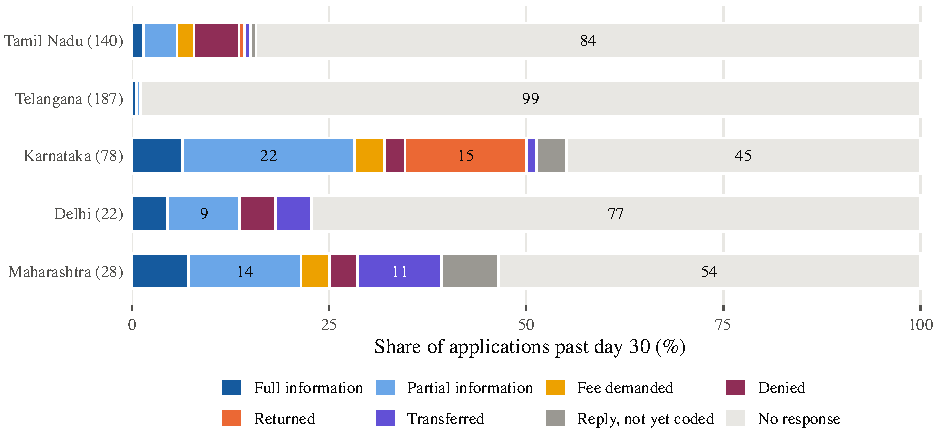
\includegraphics[width=\textwidth]{figures/fig_outcomes.pdf}
\begin{minipage}{\textwidth}\footnotesize
\textit{Notes:} Applications past day 30, status as of 29 October, whenever the reply came. N in parentheses; segments of 8\% or more are labeled. First-pass coding of reply documents, not yet double-coded. Telangana is a lower bound because its portal sends no status emails.
\end{minipage}
\end{figure}

\FloatBarrier
\begin{figure}[!htbp]
\centering
\caption{Time to first response, by state}
\label{fig:fig_km_state}
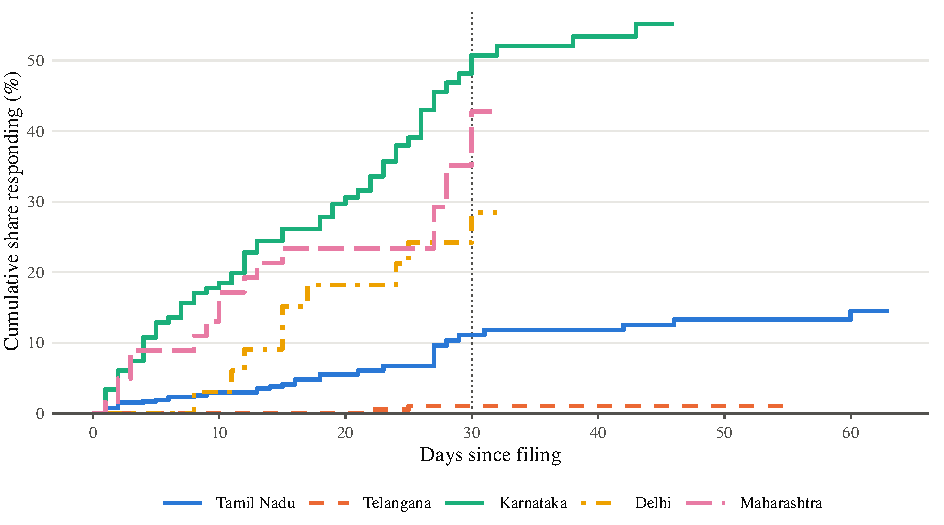
\includegraphics[width=\textwidth]{figures/fig_km_state.pdf}
\begin{minipage}{\textwidth}\footnotesize
\textit{Notes:} Kaplan-Meier estimates of time to any response (any office action, including a transfer or fee demand), all 999 dated filings, censored at 29 October; curves stop when fewer than 10 applications remain at risk. Dotted line: the 30-day limit in s.7(1). Telangana is a lower bound because its portal sends no status emails.
\end{minipage}
\end{figure}

\FloatBarrier
\begin{table}[!htbp]
\centering
\caption{How fast offices respond}
\label{tab:tab_speed}
\small
\begin{threeparttable}
\begin{tabular}{lrrrrrr}
\toprule
& \multicolumn{5}{c}{Days since filing} & \multicolumn{1}{c}{Responders:} \\ \cmidrule(lr){2-6} State & 7 & 14 & 21 & 30 & 45 & median days / N \\
\midrule
\addlinespace\multicolumn{7}{l}{\textit{Panel A. Any response by this day (\%)}} \\
Tamil Nadu & 2.5 & 3.7 & 6.4 & 12.9 & 14.3 & 14 \\
Telangana & 0.0 & 0.0 & 0.0 & 1.1 & 0.0 & 24 \\
Karnataka & 15.4 & 24.2 & 32.4 & 51.3 & 55.0 & 12 \\
Delhi & 0.0 & 9.1 & 18.2 & 22.7 &  & 15 \\
Maharashtra & 10.2 & 22.4 & 24.5 & 46.4 &  & 11 \\
All excl. Telangana & 5.5 & 10.2 & 16.9 & 28.4 & 23.3 & 13 \\
\addlinespace\multicolumn{7}{l}{\textit{Panel B. Applications exposed at least this long (N)}} \\
Tamil Nadu & 482 & 355 & 188 & 140 & 140 & 35 \\
Telangana & 209 & 188 & 187 & 187 & 138 & 2 \\
Karnataka & 143 & 124 & 102 & 78 & 40 & 62 \\
Delhi & 33 & 33 & 33 & 22 & 0 & 9 \\
Maharashtra & 49 & 49 & 49 & 28 & 0 & 18 \\
All excl. Telangana & 707 & 561 & 372 & 268 & 180 & 124 \\
\bottomrule
\end{tabular}
\begin{tablenotes}[flushleft]\footnotesize
\item \textit{Notes:} All dated filings; each column uses only applications filed at least that long ago, so shares need not rise. Any response: any office action, including a transfer or fee demand. Blank: fewer than 10 applications. Last column: median days (Panel A), responders (Panel B).
\end{tablenotes}
\end{threeparttable}
\end{table}

\FloatBarrier
\begin{table}[!htbp]
\centering
\caption{Any response within 30 days, by letter (raw comparison)}
\label{tab:tab_response_letter}
\small
\begin{threeparttable}
\begin{tabular}{lrrrrrr}
\toprule
& \multicolumn{2}{c}{Plain} & \multicolumn{2}{c}{Legal salience} & & \\ \cmidrule(lr){2-3}\cmidrule(lr){4-5} State & N & \% & N & \% & Difference & Fisher $p$ \\
\midrule
Tamil Nadu & 93 & 12.9 & 47 & 12.8 & $-$0.1 & 1.000 \\
Telangana & 130 & 1.5 & 57 & 0.0 & $-$1.5 & 1.000 \\
Karnataka & 52 & 48.1 & 26 & 57.7 & 9.6 & 0.477 \\
Delhi & 15 & 20.0 & 7 & 28.6 & 8.6 & 1.000 \\
Maharashtra & 20 & 45.0 & 8 & 50.0 & 5.0 & 1.000 \\
\midrule
All states & 310 & 16.5 & 145 & 18.6 & 2.2 & 0.594 \\
All excl. Telangana & 180 & 27.2 & 88 & 30.7 & 3.5 & 0.566 \\
\bottomrule
\end{tabular}
\begin{tablenotes}[flushleft]\footnotesize
\item \textit{Notes:} Applications past day 30. Legal salience: the letter adds the s.7(1) deadline and s.20 penalties to the plain request. Any response: any office action, including a transfer or fee demand. Raw differences in percentage points; the Tamil Nadu row is confounded with tier. Interim, unregistered look.
\end{tablenotes}
\end{threeparttable}
\end{table}

\FloatBarrier
\begin{figure}[!htbp]
\centering
\caption{Time to first response, by letter}
\label{fig:fig_km_letter}
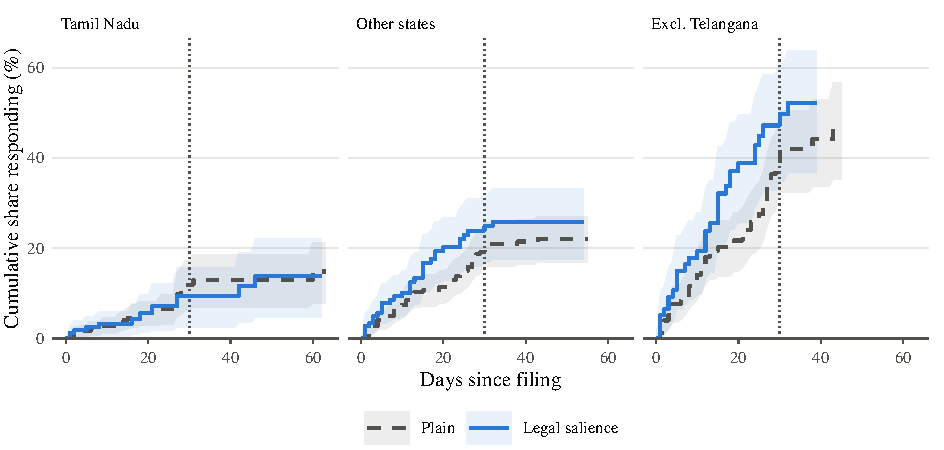
\includegraphics[width=\textwidth]{figures/fig_km_letter.pdf}
\begin{minipage}{\textwidth}\footnotesize
\textit{Notes:} Kaplan-Meier estimates of time to any response (any office action, including a transfer or fee demand) with 95\% bands, all filings, raw, so the Tamil Nadu panel is confounded with tier. Legal salience: the letter adds the s.7(1) deadline and s.20 penalties. Excl. Telangana: Karnataka, Delhi and Maharashtra. Dotted line: day 30.
\end{minipage}
\end{figure}

\FloatBarrier
\begin{table}[!htbp]
\centering
\caption{Response by Tamil Nadu tier and by filing cohort (\%)}
\label{tab:tab_cuts}
\small
\begin{threeparttable}
\begin{tabular}{lrrrr}
\toprule
Group & N & Any response & Reply & Information supplied \\
\midrule
\addlinespace\multicolumn{5}{l}{\textit{Panel A. Tamil Nadu by tier, by day 30}} \\
Department & 7 & 28.6 & 28.6 & 28.6 \\
Head of Department & 21 & 42.9 & 38.1 & 14.3 \\
Sub Office & 112 & 6.2 & 6.2 & 1.8 \\
\addlinespace\multicolumn{5}{l}{\textit{Panel B. By filing cohort, by day 14}} \\
Tamil Nadu, filed by 30 September & 140 & 5.0 & 4.3 & 2.1 \\
Tamil Nadu, filed in October & 213 & 2.3 & 0.5 & 0.0 \\
Telangana, filed by 30 September & 187 & 0.0 & 0.0 & 0.0 \\
Telangana, filed in October & 1 &  &  &  \\
Karnataka, filed by 30 September & 78 & 23.1 & 21.8 & 10.3 \\
Karnataka, filed in October & 45 & 26.7 & 24.4 & 6.7 \\
Delhi, filed by 30 September & 28 & 10.7 & 10.7 & 10.7 \\
Delhi, filed in October & 5 &  &  &  \\
Maharashtra, filed by 30 September & 36 & 25.0 & 16.7 & 11.1 \\
Maharashtra, filed in October & 13 & 15.4 & 15.4 & 15.4 \\
\bottomrule
\end{tabular}
\begin{tablenotes}[flushleft]\footnotesize
\item \textit{Notes:} Any response: any office action, including a transfer or fee demand. Reply: excludes transfers. Information supplied: coded full or partial. Panel A: past day 30, from only 11 of 40 departments because of filing order. Panel B: filed at least 14 days ago; blank cells have fewer than 10 applications.
\end{tablenotes}
\end{threeparttable}
\end{table}

\FloatBarrier
\begin{figure}[!htbp]
\centering
\caption{Any response within 30 days, by government function}
\label{fig:fig_function}
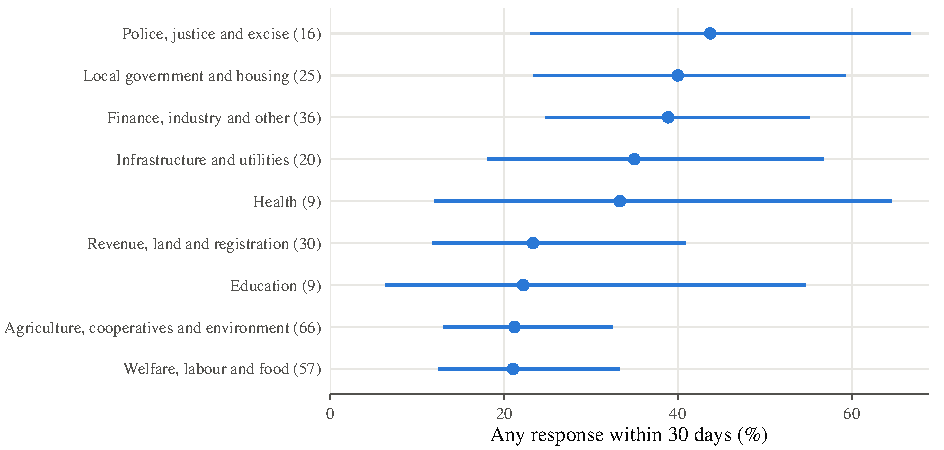
\includegraphics[width=\textwidth]{figures/fig_function.pdf}
\begin{minipage}{\textwidth}\footnotesize
\textit{Notes:} Applications past day 30, excluding Telangana. N in parentheses; bars are Wilson 95\% intervals. Any response: any office action, including a transfer or fee demand. Function is keyword-coded from department and office names (crosswalk in data/cleaned/). Pooled across states, so state differences are not removed.
\end{minipage}
\end{figure}

\FloatBarrier
\begin{table}[!htbp]
\centering
\caption{Any response within 30 days, by filer group}
\label{tab:tab_filer}
\small
\begin{threeparttable}
\begin{tabular}{lrrrrrr}
\toprule
& \multicolumn{2}{c}{RA1 and RA3} & \multicolumn{2}{c}{RA2 and RA4} & \multicolumn{2}{c}{Within block} \\ \cmidrule(lr){2-3}\cmidrule(lr){4-5}\cmidrule(lr){6-7} State & N & \% & N & \% & Difference & (SE) \\
\midrule
Tamil Nadu & 75 & 10.7 & 65 & 15.4 & $-$3.8 & (5.3) \\
Telangana & 124 & 1.6 & 63 & 0.0 & $-$1.6 & (1.1) \\
Karnataka & 28 & 57.1 & 50 & 50.0 & $-$7.1 & (11.9) \\
Delhi & 11 & 27.3 & 11 & 18.2 & $-$9.1 & (18.6) \\
Maharashtra & 12 & 33.3 & 16 & 56.2 & 22.9 & (19.1) \\
\midrule
All states & 250 & 13.2 & 205 & 22.4 & $-$2.0 & (3.1) \\
All excl. Telangana & 126 & 24.6 & 142 & 32.4 & $-$2.2 & (5.3) \\
\bottomrule
\end{tabular}
\begin{tablenotes}[flushleft]\footnotesize
\item \textit{Notes:} Applications past day 30. Any response: any office action, including a transfer or fee demand. Only RA2 and RA4 could receive calls and both are one person, so this bundles phone with name and address. Difference: coefficient on RA2/RA4 with block fixed effects and robust SE, in percentage points.
\end{tablenotes}
\end{threeparttable}
\end{table}

\FloatBarrier
\begin{table}[!htbp]
\centering
\caption{What the coded replies contain}
\label{tab:tab_content}
\small
\begin{threeparttable}
\begin{tabular}{lrrrr}
\toprule
 & Tamil Nadu (26) & Others (78) & All (104) & All (\%) \\
\midrule
\addlinespace\multicolumn{5}{l}{\textit{Disposition}} \\
\quad Full information & 4 & 23 & 27 & 26 \\
\quad Partial information & 4 & 16 & 20 & 19 \\
\quad Fee asked first & 6 & 12 & 18 & 17 \\
\quad Denied or deflected & 6 & 4 & 10 & 10 \\
\quad Returned & 1 & 15 & 16 & 15 \\
\quad Transferred & 5 & 8 & 13 & 12 \\
\addlinespace\multicolumn{5}{l}{\textit{Data supplied}} \\
\quad Application-level register & 5 & 21 & 26 & 25 \\
\quad Monthly or category counts & 1 & 5 & 6 & 6 \\
\quad Period totals & 4 & 11 & 15 & 14 \\
\quad Prose only & 0 & 2 & 2 & 2 \\
\quad None & 16 & 39 & 55 & 53 \\
\addlinespace\multicolumn{5}{l}{\textit{Section 25 annual return}} \\
\quad Supplied & 3 & 15 & 18 & 17 \\
\quad Not held & 3 & 3 & 6 & 6 \\
\quad Offered on payment & 5 & 4 & 9 & 9 \\
\quad Told to apply separately & 0 & 2 & 2 & 2 \\
\quad Referred to website & 1 & 1 & 2 & 2 \\
\quad Not addressed & 14 & 53 & 67 & 64 \\
\addlinespace\multicolumn{5}{l}{\textit{How it arrived}} \\
\quad Post & 17 & 34 & 51 & 49 \\
\quad Portal & 8 & 26 & 34 & 33 \\
\quad Email & 1 & 18 & 19 & 18 \\
\addlinespace\multicolumn{5}{l}{\textit{Provisions cited}} \\
\quad Exemption, s.8 & 0 & 2 & 2 & 2 \\
\quad Sections 2(f) or 7(9) & 6 & 4 & 10 & 10 \\
\quad Transfer, s.6(3) & 0 & 7 & 7 & 7 \\
\quad None & 19 & 64 & 83 & 80 \\
\bottomrule
\end{tabular}
\begin{tablenotes}[flushleft]\footnotesize
\item \textit{Notes:} All 104 coded replies, whenever they came. First-pass coding, not yet double-coded. Fees were quoted in 15 replies (median Rs 40, maximum Rs 832).
\end{tablenotes}
\end{threeparttable}
\end{table}

\FloatBarrier
\begin{table}[!htbp]
\centering
\caption{Office phone calls to the filer, RA2 and RA4 filings only}
\label{tab:tab_calls}
\small
\begin{threeparttable}
\begin{tabular}{lrrrrr}
\toprule
& & & & \multicolumn{2}{c}{Calls / filings} \\ \cmidrule(lr){5-6} State & Filings & Calls & Per 100 filings & Plain & Legal \\
\midrule
\addlinespace\multicolumn{6}{l}{\textit{Panel A. By state}} \\
Tamil Nadu & 267 & 2 & 0.7 & 1 / 185 & 1 / 82 \\
Telangana & 94 & 0 & 0.0 & 0 / 65 & 0 / 29 \\
Karnataka & 86 & 1 & 1.2 & 1 / 60 & 0 / 26 \\
Delhi & 22 & 1 & 4.5 & 1 / 16 & 0 / 6 \\
Maharashtra & 32 & 5 & 15.6 & 5 / 22 & 0 / 10 \\
\midrule
All & 501 & 9 & 1.8 & 8 / 348 & 1 / 153 \\
\addlinespace\multicolumn{6}{l}{\textit{Panel B. Why the office called}} \\
\quad Clarify what is sought &  & 3 &  &  &  \\
\quad Ask why the filer applied &  & 3 &  &  &  \\
\quad Give an answer by phone &  & 2 &  &  &  \\
\quad Confirm a reply arrived &  & 1 &  &  &  \\
\bottomrule
\end{tabular}
\begin{tablenotes}[flushleft]\footnotesize
\item \textit{Notes:} Only RA2 and RA4 could receive calls, so other filings are excluded and calls never enter response rates. Taken from RA notes up to 29 October, so possibly undercounted. The Act requires no reason from the applicant (s.6(2)).
\end{tablenotes}
\end{threeparttable}
\end{table}

\FloatBarrier
\begin{table}[!htbp]
\centering
\caption{Does the letter predict who is filed and who has reached day 30?}
\label{tab:tab_balance}
\small
\begin{threeparttable}
\begin{tabular}{lrrrrrrr}
\toprule
& & \multicolumn{3}{c}{Filed (\%)} & \multicolumn{3}{c}{Past day 30 (\%)} \\ \cmidrule(lr){3-5}\cmidrule(lr){6-8} State & N & Plain & Legal & $p$ & Plain & Legal & $p$ \\
\midrule
\addlinespace\multicolumn{8}{l}{\textit{Panel A. All drawn applications}} \\
Tamil Nadu & 1,000 & 52.0 & 53.7 & 0.867 & 13.3 & 15.7 & 0.901 \\
Telangana & 375 & 57.6 & 59.3 & 0.702 & 49.6 & 50.4 & 0.774 \\
Karnataka & 180 & 81.7 & 83.3 & 0.797 & 41.3 & 48.1 & 0.399 \\
Delhi & 44 & 100.0 & 100.0 &  & 50.0 & 50.0 &  \\
Maharashtra & 66 & 93.5 & 90.0 & 0.641 & 43.5 & 40.0 & 0.641 \\
\midrule
\addlinespace\multicolumn{8}{l}{\textit{Panel B. Tamil Nadu past day 30, by tier}} \\
 & N & Plain & Legal &  & Legal (\%) & Drawn (\%) &  \\
Department & 7 & 0 & 7 &  & 100.0 & 32.5 &  \\
Head of Department & 21 & 15 & 6 &  & 28.6 & 25.7 &  \\
Sub Office & 112 & 78 & 34 &  & 30.4 & 30.6 &  \\
\bottomrule
\end{tabular}
\begin{tablenotes}[flushleft]\footnotesize
\item \textit{Notes:} Past day 30: filed by 29 September. Panel A: $p$-values on the letter in a linear probability model with randomization-block fixed effects and robust SEs. Panel B: counts, with the legal share among them and among all drawn in that tier. All 7 department-tier filings past day 30 got the legal letter.
\end{tablenotes}
\end{threeparttable}
\end{table}

\FloatBarrier
\begin{table}[!htbp]
\centering
\caption{Effect of the legal-salience letter}
\label{tab:tab_main}
\small
\begin{threeparttable}
\begin{tabular}{lrrrrrr}
\toprule
& \multicolumn{2}{c}{Tamil Nadu} & \multicolumn{2}{c}{Other states} & \multicolumn{2}{c}{Excl. Telangana} \\ \cmidrule(lr){2-3}\cmidrule(lr){4-5}\cmidrule(lr){6-7}  & (1) & (2) & (3) & (4) & (5) & (6) \\
\midrule
\addlinespace\multicolumn{7}{l}{\textit{Panel A. Any response by day 30}} \\
Legal letter & $-$0.1 & 1.1 & 2.6 & 7.0 & 8.5 & 31.3 \\
 & (6.0) & (5.8) & (3.9) & (3.8) & (9.4) & (13.5) \\
Plain-letter mean & 12.9 & 9.1 & 18.0 & 12.0 & 42.5 & 39.1 \\
Detectable effect (2.8 $\times$ SE) & 16.9 & 16.2 & 10.9 & 10.6 & 26.3 & 37.8 \\
Randomization-inference $p$ &  & 1.000 & 0.569 & 0.144 & 0.440 & 0.069 \\
N & 140 & 128 & 315 & 242 & 128 & 73 \\
\addlinespace\multicolumn{7}{l}{\textit{Panel B. Reply by day 30}} \\
Legal letter & 2.0 & 2.3 & 2.8 & 6.3 & 8.9 & 28.3 \\
 & (5.9) & (5.6) & (3.9) & (3.6) & (9.2) & (13.0) \\
Plain-letter mean & 10.8 & 8.0 & 15.7 & 10.8 & 36.8 & 34.8 \\
Detectable effect (2.8 $\times$ SE) & 16.4 & 15.7 & 10.8 & 10.1 & 25.9 & 36.4 \\
Randomization-inference $p$ &  & 0.703 & 0.551 & 0.174 & 0.415 & 0.125 \\
N & 140 & 128 & 315 & 242 & 128 & 73 \\
\addlinespace\multicolumn{7}{l}{\textit{Panel C. Information supplied by day 30}} \\
Legal letter & 0.0 & $-$0.6 & $-$3.5 & $-$0.9 & $-$6.2 & 0.5 \\
 & (3.6) & (3.4) & (3.1) & (2.9) & (7.5) & (10.8) \\
Plain-letter mean & 4.3 & 3.4 & 10.1 & 7.2 & 23.0 & 21.7 \\
Detectable effect (2.8 $\times$ SE) & 10.2 & 9.5 & 8.8 & 8.0 & 21.0 & 30.3 \\
Randomization-inference $p$ &  & 1.000 & 0.366 & 1.000 & 0.486 & 1.000 \\
N & 140 & 128 & 315 & 242 & 128 & 73 \\
\midrule
Randomization-block FE & No & Yes & Yes & Yes & Yes & Yes \\
Department-group FE & No & No & No & Yes & No & Yes \\
\bottomrule
\end{tabular}
\begin{tablenotes}[flushleft]\footnotesize
\item \textit{Notes:} Linear probability models, applications past day 30, percentage points, robust SEs. Legal letter: cites the s.7(1) deadline and s.20 penalties. Any response includes transfers and fee demands; reply excludes them; information: coded full or partial. Blocks: department $\times$ tier (Tamil Nadu), state $\times$ batch (others). Columns (4), (6) rest on 162, 41 applications in department groups with both letters.
\end{tablenotes}
\end{threeparttable}
\end{table}

\FloatBarrier
\begin{table}[!htbp]
\centering
\caption{Legal-salience letter: alternative specifications}
\label{tab:tab_robust}
\footnotesize
\begin{threeparttable}
\begin{tabular}{lrrrrrr}
\toprule
& \multicolumn{2}{c}{Tamil Nadu} & \multicolumn{2}{c}{Other states} & \multicolumn{2}{c}{Excl. Telangana} \\ \cmidrule(lr){2-3}\cmidrule(lr){4-5}\cmidrule(lr){6-7}  & Coef. (SE) & N & Coef. (SE) & N & Coef. (SE) & N \\
\midrule
\addlinespace\multicolumn{7}{l}{\textit{Linear probability, any response (percentage points)}} \\
Baseline, by day 30 & 1.1 (5.8) & 128 & 2.6 (3.9) & 315 & 8.5 (9.4) & 128 \\
By day 35 & $-$0.1 (5.9) & 128 & 3.2 (3.7) & 269 & 13.3 (11.5) & 82 \\
By day 45 & 2.3 (5.6) & 128 & 3.5 (4.0) & 178 & 14.3 (16.5) & 40 \\
By day 14, all exposed that long & $-$0.5 (1.6) & 323 & 3.4 (3.4) & 393 & 6.5 (6.5) & 206 \\
Adding RA fixed effects & 1.2 (5.8) & 128 & 2.8 (3.9) & 315 & 8.9 (9.5) & 128 \\
Adding filing-week fixed effects & 1.3 (5.8) & 128 & 3.1 (3.9) & 315 & 11.1 (9.3) & 128 \\
Excluding Maharashtra (shorter letter) &  &  & 2.4 (3.8) & 287 & 9.4 (10.4) & 100 \\
RA2 and RA4 filings only & 4.3 (8.6) & 57 & $-$1.2 (6.6) & 140 & $-$2.3 (12.4) & 77 \\
RA1 and RA3 filings only & 3.1 (8.0) & 65 & 4.9 (4.7) & 175 & 21.3 (14.9) & 51 \\
\addlinespace\multicolumn{7}{l}{\textit{Cox model, all filings (hazard ratio)}} \\
Legal letter, stratified by block & 1.08 (0.45) & 527 & 1.40 (0.31) & 472 & 1.45 (0.32) & 254 \\
\bottomrule
\end{tabular}
\begin{tablenotes}[flushleft]\footnotesize
\item \textit{Notes:} All rows: any response (any office action, including a transfer or fee demand), legal letter as in Table~\ref{tab:tab_main}, block fixed effects, robust SEs. Later cutoffs and the day-14 row use applications exposed that long. Filer-group rows are exploratory. The Cox model is our addition, not in the design document; its SE is on the hazard-ratio scale.
\end{tablenotes}
\end{threeparttable}
\end{table}

\FloatBarrier
\begin{figure}[!htbp]
\centering
\caption{Effect of the legal-salience letter by days since filing}
\label{fig:fig_horizon}
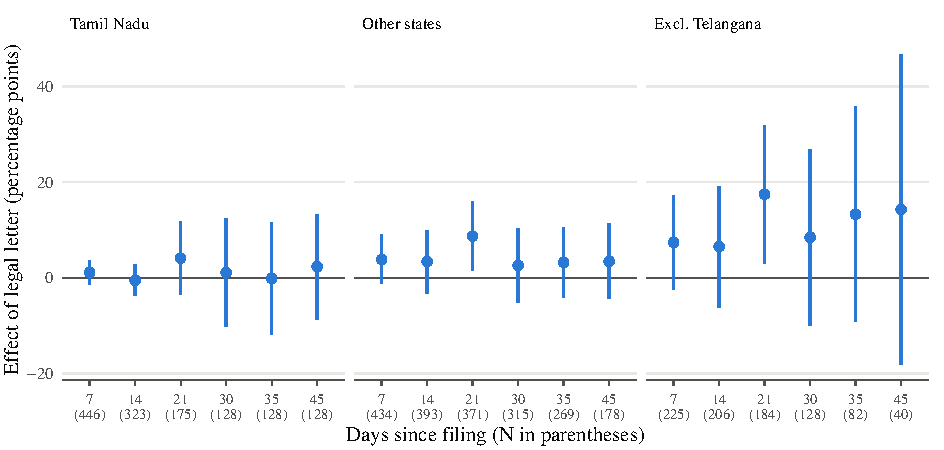
\includegraphics[width=\textwidth]{figures/fig_horizon.pdf}
\begin{minipage}{\textwidth}\footnotesize
\textit{Notes:} Each point is a separate linear probability model of any response (any office action, including a transfer or fee demand) by that day on the legal letter, with randomization-block fixed effects, on applications filed at least that long ago. Bars are 95\% intervals from robust SEs. The sample changes across horizons.
\end{minipage}
\end{figure}

\FloatBarrier
\begin{table}[!htbp]
\centering
\caption{Correlates of any response within 30 days (descriptive)}
\label{tab:tab_correlates}
\footnotesize
\begin{threeparttable}
\begin{tabular}{lccc}
\toprule
 & All excl. Telangana & Tamil Nadu & Karnataka, Delhi, Maharashtra \\
\midrule
\addlinespace\multicolumn{4}{l}{\textit{State (relative to Tamil Nadu)}} \\
\quad Karnataka & 45.1 (7.3) &  &  \\
\quad Delhi & 10.2 (12.5) &  &  \\
\quad Maharashtra & 39.8 (9.9) &  &  \\
\addlinespace\multicolumn{4}{l}{\textit{Tamil Nadu tier (relative to Sub Office)}} \\
\quad Department &  & 26.7 (17.4) &  \\
\quad Head of Department &  & 38.0 (11.0) &  \\
\addlinespace\multicolumn{4}{l}{\textit{Function (relative to finance, industry and other)}} \\
\quad Agriculture, cooperatives and environment & $-$10.6 (8.5) & 5.5 (8.9) & $-$27.1 (19.3) \\
\quad Education & $-$31.2 (17.7) &  & $-$44.3 (19.7) \\
\quad Health & $-$1.7 (18.0) & 13.8 (16.0) & $-$15.7 (26.8) \\
\quad Infrastructure and utilities & $-$3.3 (11.0) & 9.1 (11.2) & $-$4.4 (19.3) \\
\quad Local government and housing & $-$30.8 (13.1) &  & $-$49.1 (16.0) \\
\quad Police, justice and excise & $-$10.6 (13.6) &  & $-$26.6 (15.0) \\
\quad Revenue, land and registration & $-$17.0 (9.8) & 3.8 (9.7) & $-$37.4 (19.3) \\
\quad Welfare, labour and food & $-$25.0 (8.8) & $-$5.8 (9.5) & $-$47.7 (15.3) \\
\addlinespace\multicolumn{4}{l}{\textit{Application}} \\
\quad Filed by RA2 or RA4 & 4.7 (5.0) & 3.4 (5.3) & 6.5 (8.8) \\
\quad Legal letter & 6.1 (5.4) & $-$2.4 (6.1) & 15.0 (9.6) \\
\midrule
State $\times$ batch FE & No & No & Yes \\
N & 268 & 140 & 128 \\
\bottomrule
\end{tabular}
\begin{tablenotes}[flushleft]\footnotesize
\item \textit{Notes:} Linear probability models, applications past day 30, percentage points, robust SEs in parentheses. Outcome: any office action, including a transfer or fee demand. Telangana is excluded because its outcome is not comparable. Only the letter and, within state, the filer are randomized; the rest are associations. Blank function cells: no such offices past day 30.
\end{tablenotes}
\end{threeparttable}
\end{table}

\FloatBarrier
\begin{table}[!htbp]
\centering
\caption{What the original inputs cover}
\label{tab:tab_audit}
\small
\begin{threeparttable}
\begin{tabular}{lrrrrrr}
\toprule
State & Drawn & Filed & Portal ack. & Receipt & Reply PDF & Notice, no PDF \\
\midrule
Tamil Nadu & 1,000 & 525 & 367 & 525 & 27 & 4 \\
Telangana & 375 & 218 & 121 & 216 & 2 & 0 \\
Karnataka & 180 & 148 & 148 & 144 & 51 & 10 \\
Delhi & 44 & 44 & 0 & 39 & 9 & 0 \\
Maharashtra & 66 & 61 & 60 & 59 & 16 & 0 \\
\midrule
All & 1,665 & 996 & 696 & 983 & 105 & 14 \\
\bottomrule
\end{tabular}
\begin{tablenotes}[flushleft]\footnotesize
\item \textit{Notes:} Filed: a real registration number on the RA sheet or a portal acknowledgment. Notice, no PDF: the portal says disposed, returned or rejected, but the reply has not been downloaded. No status notices reached the inboxes from Telangana, Delhi or Maharashtra, so replies left only on those portals are not observed.
\end{tablenotes}
\end{threeparttable}
\end{table}

\FloatBarrier
\begin{table}[!htbp]
\centering
\caption{Reply coding: agreement between two independent coders}
\label{tab:tab_coding}
\small
\begin{threeparttable}
\begin{tabular}{lrrr}
\toprule
 & N & Agree (\%) & Kappa \\
\midrule
\addlinespace\multicolumn{4}{l}{\textit{Panel A. Agreement}} \\
Information supplied, yes or no & 104 & 92.3 & 0.85 \\
Disposition & 104 & 74.0 & 0.69 \\
Data format & 104 & 87.5 & 0.81 \\
Section 25 return & 104 & 90.4 & 0.84 \\
Reply date & 104 & 85.6 & 0.85 \\
\midrule
 &  & First pass & Adjudicated \\
\addlinespace\multicolumn{4}{l}{\textit{Panel B. Disposition counts}} \\
Full information &  & 27 & 16 \\
Partial information &  & 20 & 38 \\
Fee asked first &  & 18 & 11 \\
Denied or deflected &  & 10 & 14 \\
Returned &  & 16 & 15 \\
Transferred &  & 13 & 10 \\
\bottomrule
\end{tabular}
\begin{tablenotes}[flushleft]\footnotesize
\item \textit{Notes:} Panel A: the second coder could not see the first codes. Panel B: disagreements went to an adjudicator who could not tell the coders apart. Full now requires the Section 25 return to be answered as well, which is stricter than the first pass. Reply coding cannot be rerun, only audited.
\end{tablenotes}
\end{threeparttable}
\end{table}

\FloatBarrier
\end{document}
